%\begin{figure}[!tbp]
%\centering
%\begin{minipage}[b]{0.4\textwidth}
%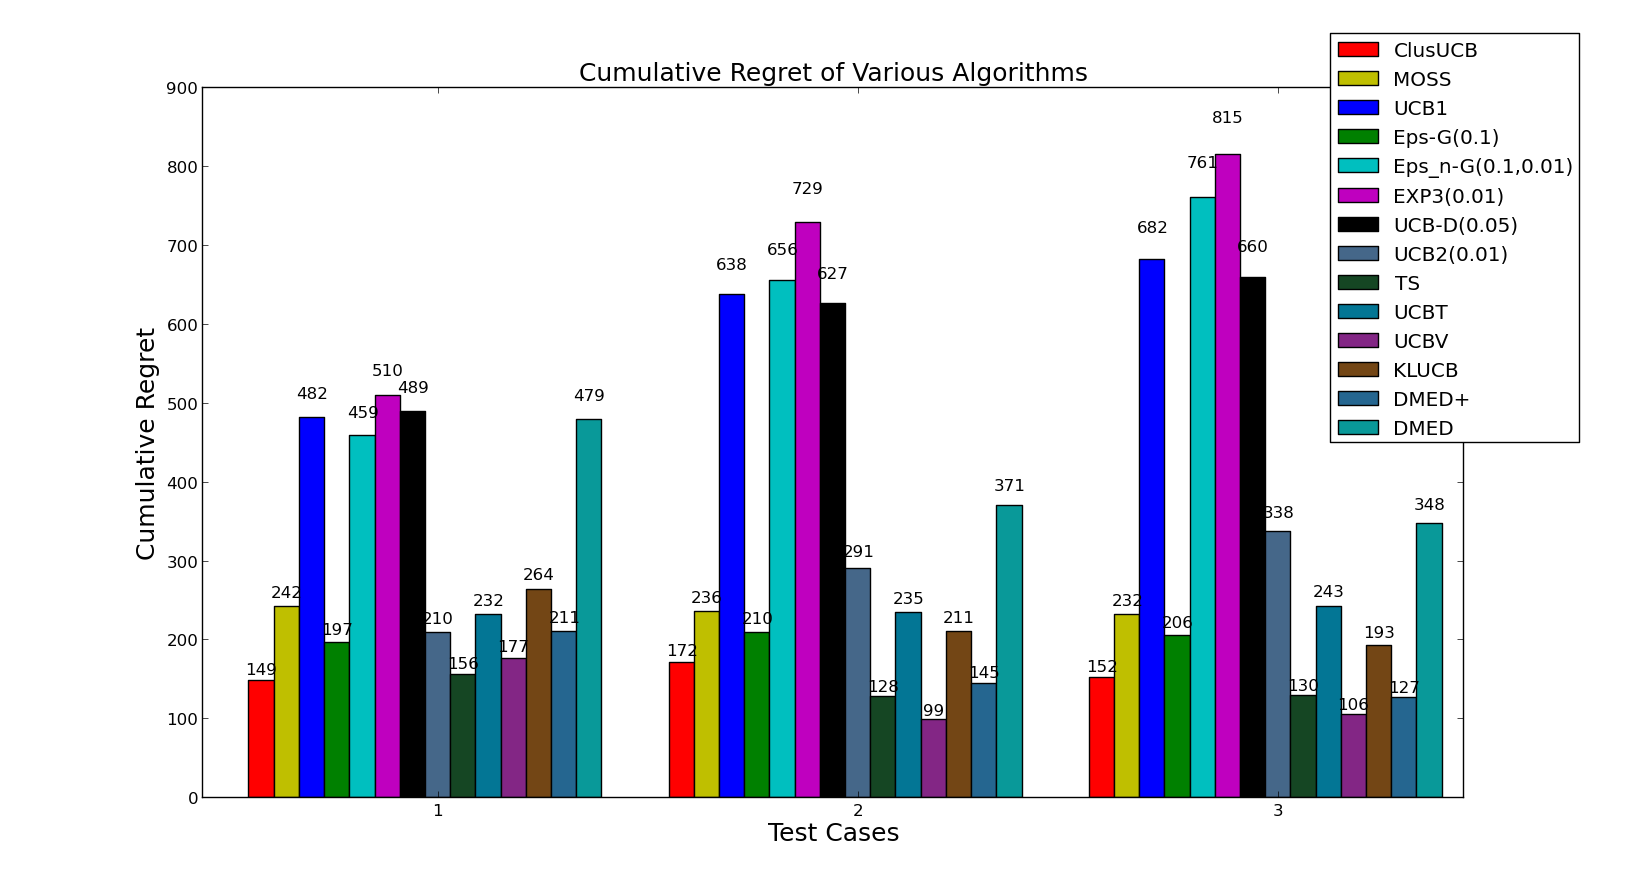
\includegraphics[width=\textwidth]{img/cl_final12.png}
%\caption{Experiment 1: Regret for various Algorithms in 3 testcases. $T=20000; \psi(m)=1.5/m$}
%\end{minipage}
%\hspace{0.1em}
%\begin{minipage}[b]{0.4\textwidth}
%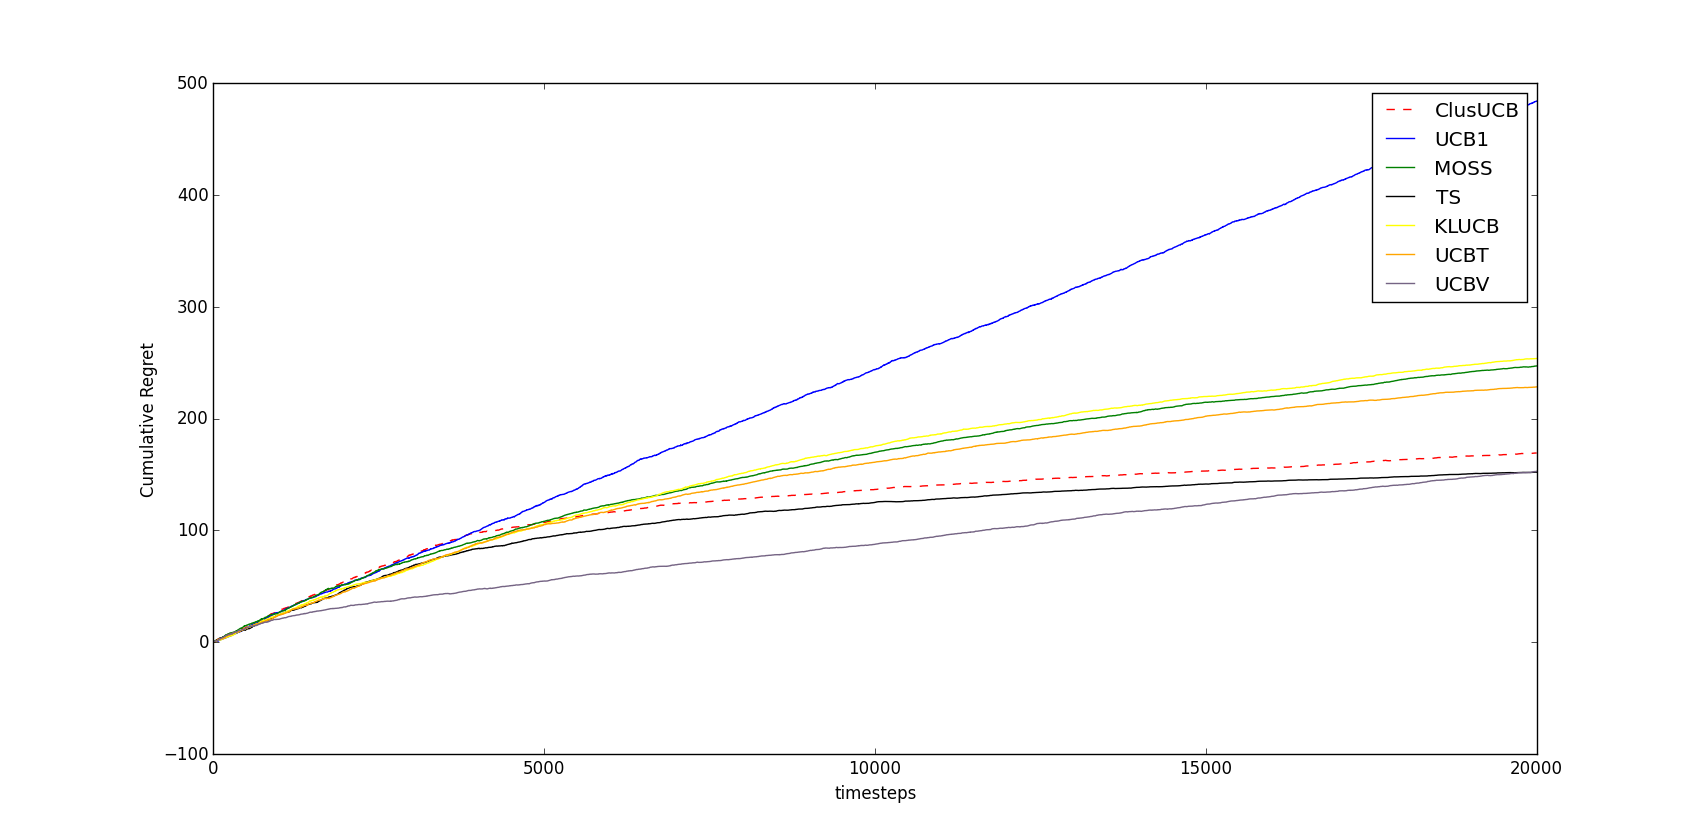
\includegraphics[width=\textwidth]{img/cl_final2.png}
%\caption{Experiment 2: Growth of Regret for test case 1. $T=20000; \psi(m)=1.5/m$}
%\end{minipage}
%\hspace{0.1em}
%\begin{minipage}[b]{0.4\textwidth}
%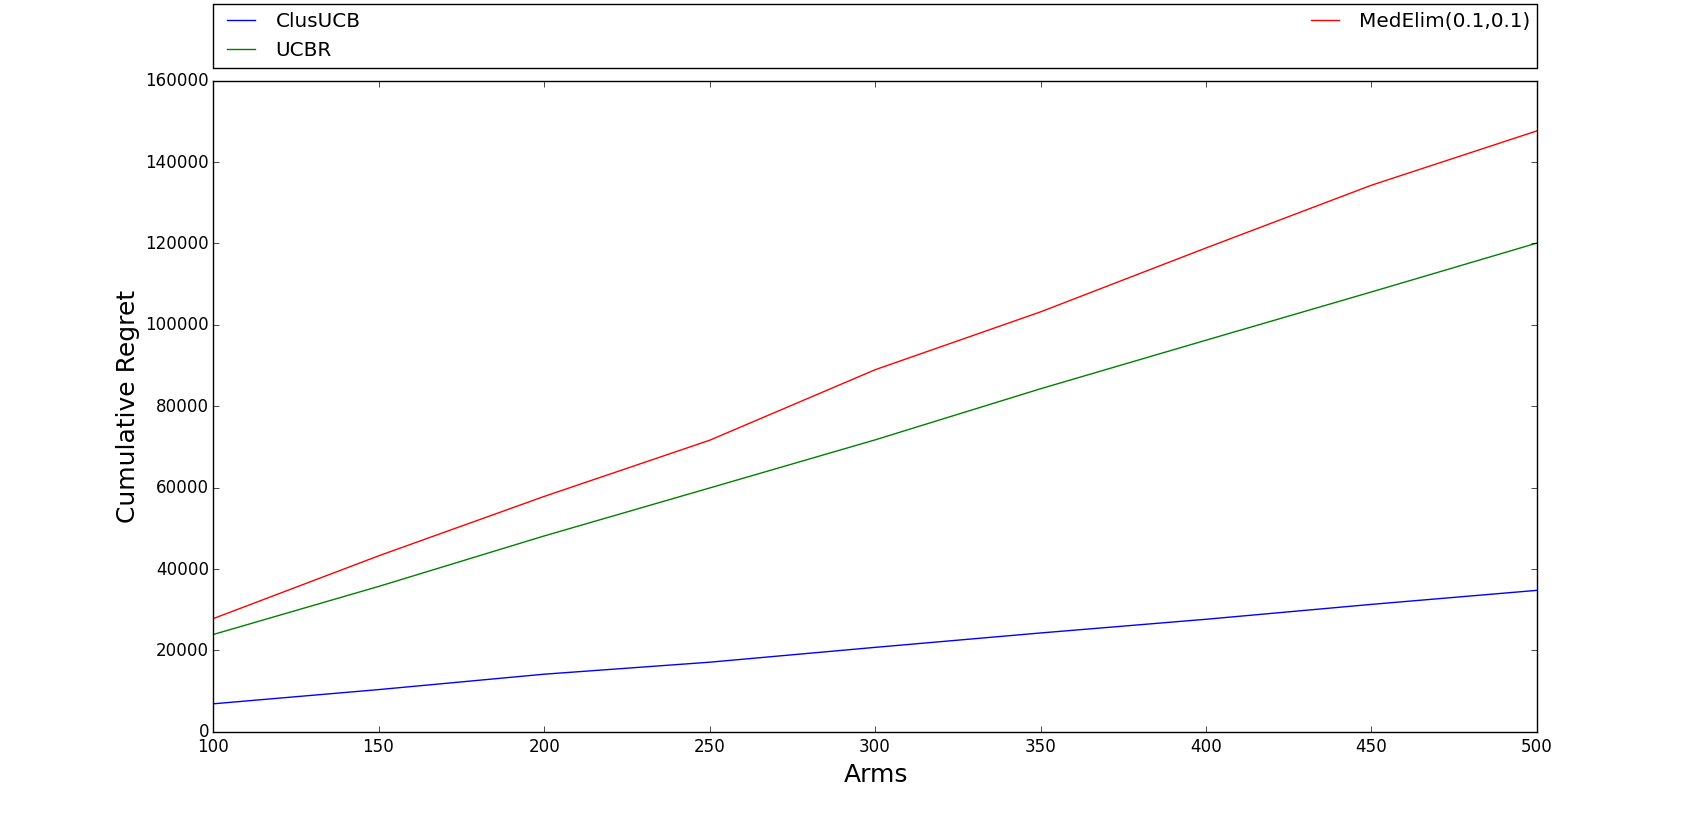
\includegraphics[width=\textwidth]{img/cl_final3.png}
%\caption{Experiment 3: Regret for ClusUCB, UCB-Improved and Median-Elimination. $T=5\times10^5; \psi(m)=0.1/m$}
%\end{minipage}
%\hspace{0.1em}
%\end{figure}
%
%%\begin{table}
%%\begin{center}
%%\begin{tabular}{|c|c|c|}
%%%\begin{figure}
%%%\vspace{1in}
%%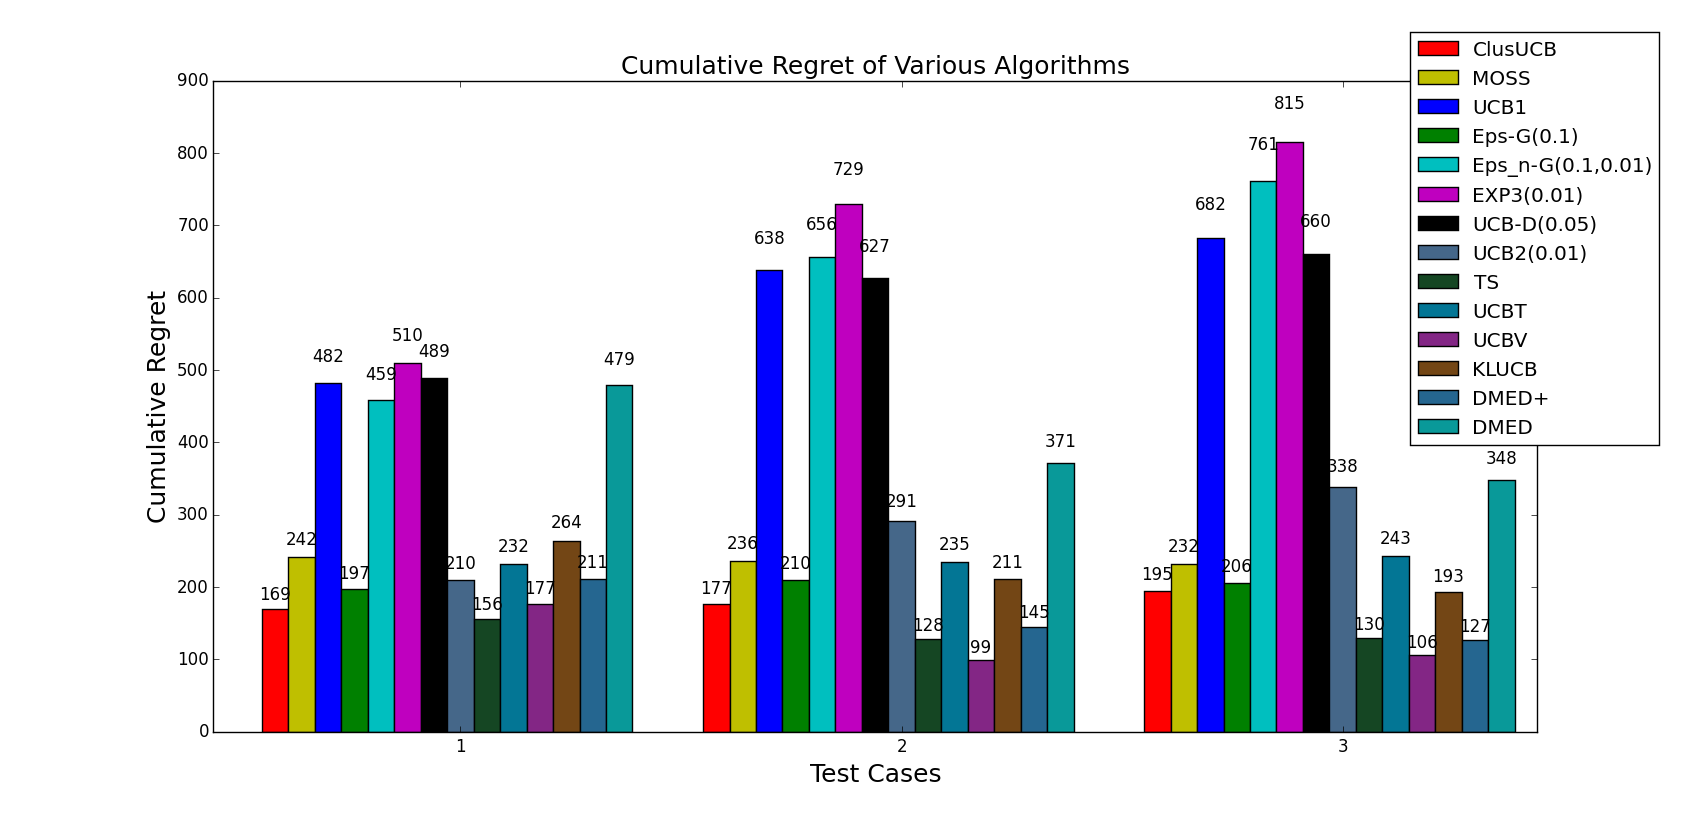
\includegraphics[scale=0.1]{img/cl_final1.png}
%%&
%%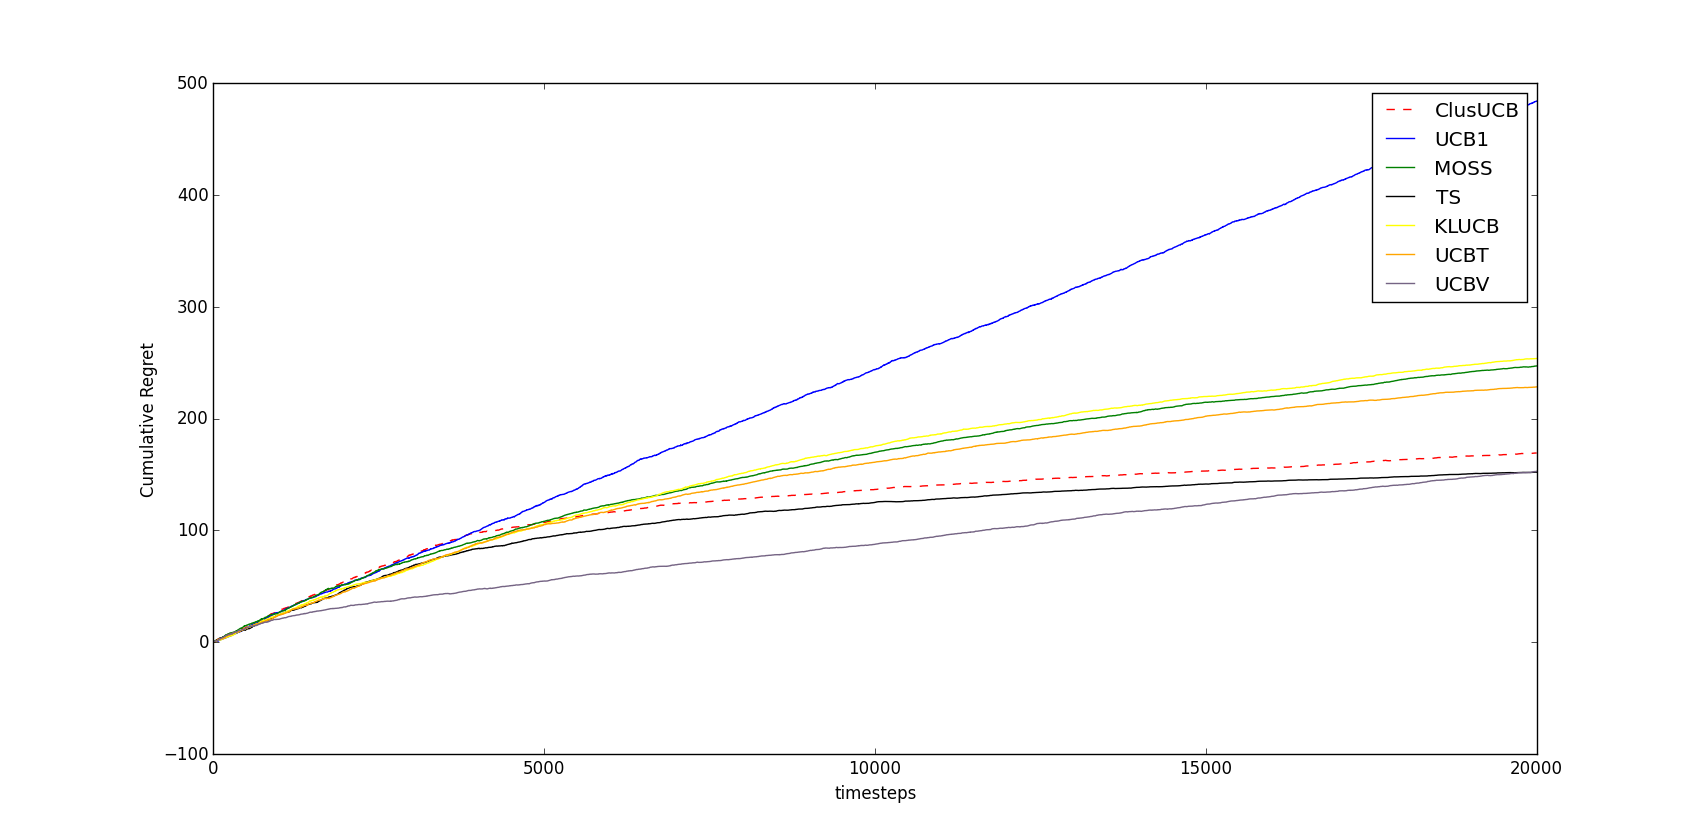
\includegraphics[scale=0.1]{img/cl_final2.png}
%%%\caption{Experiment 1: Regret for various Algorithms. $T=10000000; w=2; D=8,16; \psi(m)=K^{3/m}$}
%%& 
%%\includegraphics[scale=0.1]{img/cl_ucbr_medElim_500_1.png}
%%%\caption{Experiment 2: Regret for ClusUCB(4) and MOSS. $T=100000; w=16; D=4; \psi(m)=K^{5/m}$}
%%
%%%\end{figure}
%%\end{tabular}
%%\end{center}
%%\caption{Experiment 1: Regret for ClusUCB(4) and MOSS. $T=10^{5}; D=4,w=16; D=4,w=64; D=2,w=128; \psi(m)=K^{1/m}$}
%%\label{fig:exp1}
%%\caption{Experiment 2: Regret for ClusUCB(8) and UCB-Improved. $T=10^{7}; w=8,16 ; D=8; \psi(m)=K^{5/m}$}
%%\label{fig:exp2}
%%\caption{Experiment 3: Regret for ClusUCB(8), UCB-Improved and Median-Elimination. $T=5\times10^6; w=8; D=4; \psi(m)=K^{5/m}$}
%%\label{fig:exp3}
%%\end{table}
%
%\paragraph{}The first experiment is conducted over a testbed of $10$ arms for the 3 test-cases involving Bernoulli reward distribution with expected rewards of the arms as described below.
%\newline
%\hspace*{3em}\textbf{Test Case 1:} [0.07, 0.07, 0.07, 0.07, 0.07, 0.07, 0.07, 0.07, 0.07, 0.1]
%\newline
%\hspace*{3em}\textbf{Test Case 2:} [0.07, 0.07, 0.07, 0.05, 0.05, 0.05, 0.05, 0.05, 0.05, 0.1]
%\newline
%\hspace*{3em}\textbf{Test Case 3:} [0.07, 0.07, 0.07, 0.05, 0.05, 0.05, 0.03, 0.03, 0.03, 0.1]
%
%
%	These type of cases are frequently encountered in web-advertising domain. The regret is averaged over $50$ independent runs over each testbed and is shown in \textbf{Fig 1}. $14$ algorithms ClusUCB, MOSS, UCB1, UCB2($\alpha=0.01$), $\epsilon$-greedy($\epsilon=0.1$)(\cite{sutton1998reinforcement}), $\epsilon_{n}$-greedy($c=0.1,d=0.01$), Exp3$(\gamma=0.01)$, UCB-Delta$(\delta=0.05)$(\cite{abbasi2011improved}), UCB-Tuned, UCB-V, KL-UCB, DMED$+$, DMED(as stated in \cite{garivier2011kl}) and Thompson Sampling(\cite{agrawal2011analysis}) are run over this testbed and shown in this figure(the cumulative regret averaged over $50$ independent runs is shown above each bar). Here, we see that except Thompson Sampling and UCB-V and DMED$+$ the regret of Clustered-UCB is lower than the rest for all the test cases. Even in test case 1, the regret of ClusUCB is nearly same as Thompson Sampling and better than UCB-V and DMED$+$. In test case 1 the regret is so low for ClusUCB because $\Delta_{i}=\Delta, \forall i\in A$ and while all the algorithms employ significant exploration ClusUCB by virtue of dividing the problem into sub-problems quickly finds the optimal arm. The parameters of $\epsilon_{n}$-greedy are very difficult to estimate and if $d$ is not a tight lower bound of $\Delta$ then the result can be poor as shown in the figure. The parameter less algorithms  UCB1, MOSS, UCB-Tuned, Thompson Sampling and UCB-V are run as mentioned in the respective papers. For algorithms requiring parameters, such as UCB2, UCB-Delta, $\epsilon$-greedy, $\epsilon_{n}$-greedy, EXP3, the parameters were tried and tested over several values and then implemented in each of the test cases. KL-UCB, DMED and DMED$+$ code is taken from \cite{CapGarKau12}, and is run accordingly the way author specified with KL-UCB parameter $c=0$.  KL-UCB regret is also poorer than ClusUCB in test case 1 and 2 and same as ClusUCB in test case 3. It takes significant more time to run the algorithm than ClusUCB which might not be feasible in many real world scenarios like web advertising. In this short horizon for all the test cases ClusUCB 
%performs better than MOSS and UCB1. DMED$+$, UCB-V and TS, as expected beats ClusUCB in scenario 2 and 3. In test cases 2 and 3, ClusUCB performs bad mainly because here the $\Delta_{i}$ is much more evenly spread and ClusUCB takes significantly more exploration to find the optimal arm. Also since it's a short horizon of $T=20000$, we have taken $\psi(m)=\dfrac{1.5}{m}$.
%
%%0,4,3,3,1
%%\begin{figure}
%%%\vspace{1in}
%%\includegraphics[scale=0.25]{img/cl_moss_11_15.png}
%%\caption{Experiment 2: Regret for ClusUCB(4) and MOSS. $T=100000; w=16; D=4; \psi(m)=K^{5/m}$}
%%\label{fig:exp2}
%%\end{figure}
%
%	The second experiment is conducted over the same testbed as in test case 1 above and shown in \textbf{Fig 2}. We check the growth of regret over time for $7$ algorithms as mentioned in the figure. Here, we see that ClusUCB has a much steeper regret curve than the rest which signifies a faster exploitation and less exploration. It quickly finds the optimal arm and the cumulative regret nearly becomes negligible. UCB1 is not able to find the optimal arm in this short horizon whereas UCB-V performs much better but its regret still does not stabilize within this short horizon. TS performs well as well whereas MOSS performs much worse and hardly stabilizes in this short horizon. We also see that ClusUCB is remarkably stable in this short horizon and it outputed a sub-optimal arm only $5$ out of $50$ runs. Comparing this with UCB-V, it outputed a wrong arm $11$ out of $50$ runs. 
%%\newline
%%\begin{figure}
%%%\vspace{1in}
%%\includegraphics[scale=0.25]{img/cl_ucbr_500.png}
%%\caption{Experiment 3: Regret for ClusUCB(8) and UCB-Improved. $T=10000000; w=8,16 ; D=8; \psi(m)=K^{5/m}$}
%%\label{fig:exp3}
%%\end{figure}
%%[46, 47, 48, 50, 49]
%%[50, 50, 50, 50, 50]
%%[50, 48, 50, 50, 50]
%
%	The third experiment is conducted over a testbed of $100-500$ arms at an interval of $50$ arms, of which (for any particular run) $\frac{1}{3}$ arms have Gaussian reward distribution  $N(\mu =0.2,\sigma =0.3)$, rest $\frac{2}{3}$ arms have Gaussian reward distribution  $N(\mu =0.7,\sigma =0.3)$ and the optimal arm have parameters $N(\mu =0.9,\sigma =0.3)$. We conduct this experiment to not only check the performance of ClusUCB in Gaussian distribution, but also the growth of regret over a large set of arms. Here, we employ only select algorithms(round based algorithms) since the action space is very large and the other algorithms will take a long time to converge on the optimal arm. The regret is averaged over $50$ independent runs over this testbed and is shown in \textbf{Fig 3}. Three round-based algorithms ClusUCB, UCB-Improved and Median Elimination are run over this testbed and shown in the figure. Here, Median-Elimination performs worse than UCB-Improved. We also see that over this large set of arms 
%the regret of ClusUCB is not only much lesser than UCB-Improved and Median-Elimination but also being a round based algorithm it is much faster than other standard algorithms. Again since it's a  large horizon of $T=5\times 10^{5}$ so we have taken $\psi(m)=\dfrac{0.1}{m}$.

%10/50
%\begin{figure}
%%\vspace{1in}
%\includegraphics[scale=0.25]{img/cl_ucbr_medElim_500_1.png}
%\caption{Experiment 3: Regret for ClusUCB(8) and UCB-Improved. $T=5000000; w=8; D=4; \psi(m)=K^{5/m}$}
%\label{fig:exp3}
%\end{figure}

%[40, 42, 45, 46, 40]
%[50, 50, 50, 50, 49]
%[50, 50, 50, 50, 50]


%ABOVE OLD EXPT

\begin{figure}[!tbp]
\centering
\begin{minipage}[b]{0.4\textwidth}

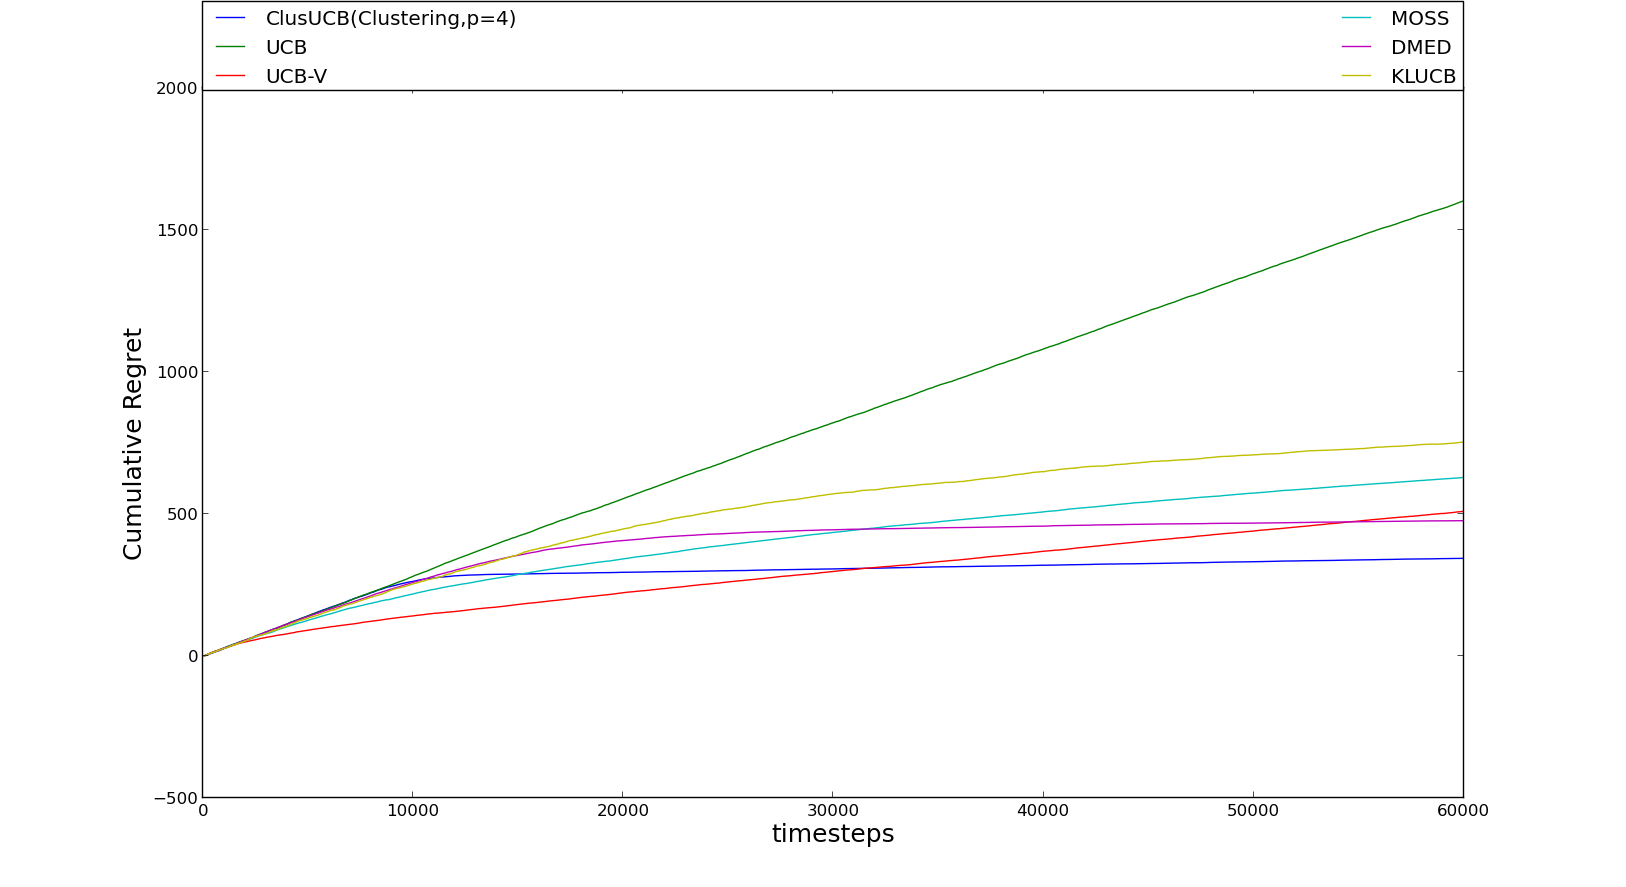
\includegraphics[width=\textwidth]{img/ClusUCB_variousAlgo.png}
\label{fig:1}
\caption{Experiment 1: Regret for various Algorithms. $T=60000$}
\end{minipage}
\hspace{0.1em}
%\begin{minipage}[b]{0.4\textwidth}
%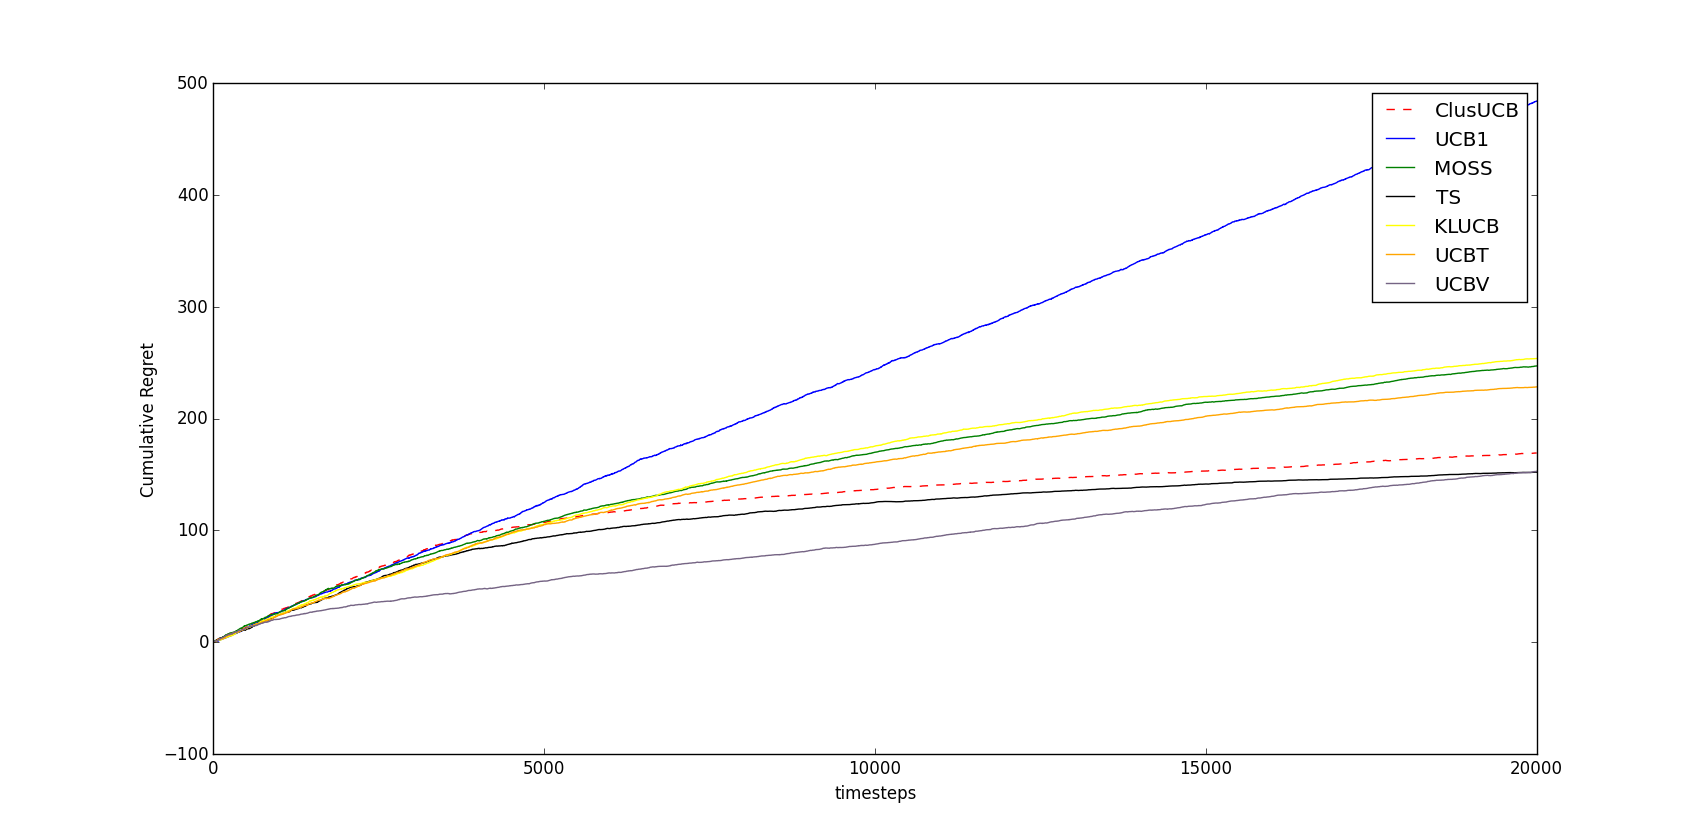
\includegraphics[width=\textwidth]{img/cl_final2.png}
%\caption{Experiment 2: Growth of Regret for test case 1. $T=20000; \psi(m)=1.5/m$}
%\end{minipage}
%\hspace{0.1em}
%\begin{minipage}[b]{0.4\textwidth}
%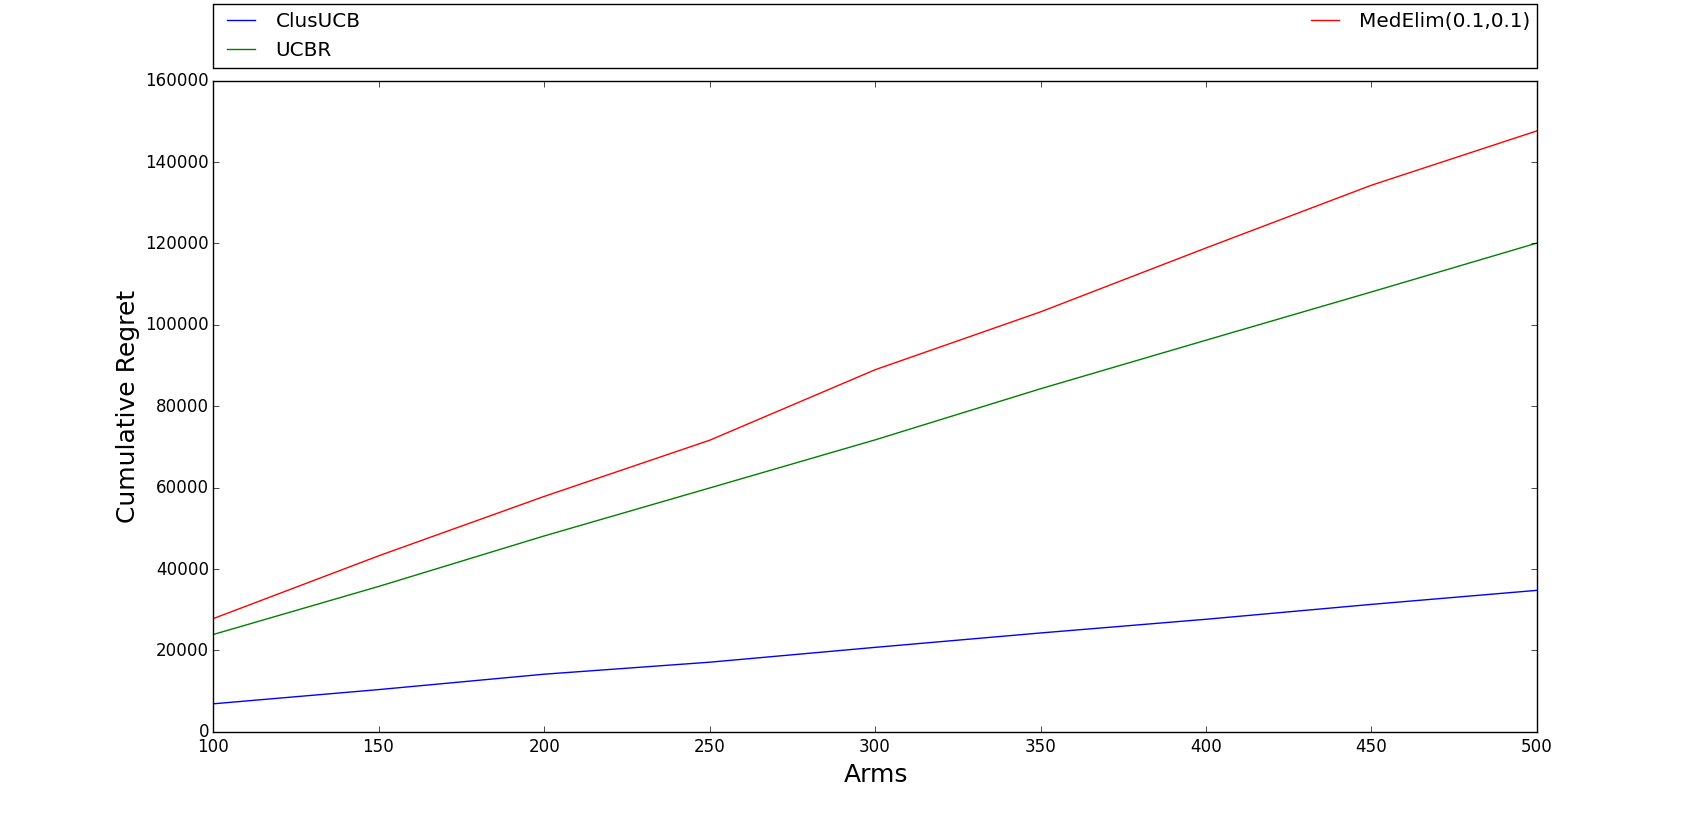
\includegraphics[width=\textwidth]{img/cl_final3.png}
%\caption{Experiment 3: Regret for ClusUCB, UCB-Improved and Median-Elimination. $T=5\times10^5; \psi(m)=0.1/m$}
%\end{minipage}
%\hspace{0.1em}
\end{figure}

\paragraph{}In the stochastic bandit literature there are several powerful algorithms with and without proven regret bounds. Algorithms like $\epsilon$-greedy(\cite{sutton1998reinforcement}) or softmax(\cite{sutton1998reinforcement}) or UCB-Tuned(\cite{auer2002finite}) has no proven regret bounds. Again algorithms like UCB-$\delta$(\cite{abbasi2011improved}) with proven regret bound better than UCB1  falls within the realm of fixed confidence setting whereas one has to provide the probability of error $\delta$. We also make a distinction between frequentist based approach like the UCB algorithms and the Bayesian approach like the Thompson Sampling(\cite{agrawal2011analysis}). We will not be experimenting against these algorithms but focus on the more recent, algorithms like KL-UCB, DMED, MOSS, UCB1, UCB-V, etc. 

\paragraph{}The first experiment is conducted over a testbed of $20$ arms for the test-cases involving Bernoulli reward distribution with expected rewards of the arms $r_{i_{a_{i}\neq a^{*}}}=0.07$ and $r^{*}=0.1$. These type of cases are frequently encountered in web-advertising domain. The horizon is set for $T=60000$ and the parameters of ClusUCB are $p=4,\psi_{m}=\log T$\textbf{(Appendix D, Definition 4)} and $\rho_{s}=\dfrac{1}{2^{2m+1}},\rho_{a}=\dfrac{1}{2^{4m+1}}$\textbf{(Appendix E, Definition 5)}, where $m$ is the round number. The regret is averaged over $100$ independent runs over each testbed and is shown in \textbf{Figure 1}. $6$ algorithms, ClusUCB, MOSS, UCB1, UCB-V, KL-UCB, DMED are run over this testbed and shown in this figure. Here, we see that ClusUCB performs better than all the algorithms mentioned above.


